\documentclass{article}
\usepackage[preprint,nonatbib]{neurips_2026}
\usepackage[T1]{fontenc}
\usepackage{amsmath,amssymb,graphicx,booktabs}
\usepackage[hidelinks]{hyperref}
% Generated by code/build_report_assets.py from data/*.json
\newcommand{\FIDvalue}{283.72}
\newcommand{\ISvalue}{2.095}
\newcommand{\ISreal}{2.284}
\newcommand{\ISsplitmean}{2.045}
\newcommand{\ISsplitstd}{0.188}
\newcommand{\ProbFID}{0.1395}
\newcommand{\SelectedEpoch}{45}
\newcommand{\BestVal}{9,059.32}
\newcommand{\TrainFirst}{10,411.04}
\newcommand{\TrainLast}{9,431.28}
\newcommand{\ValLast}{9,061.96}
\newcommand{\ParamCount}{7,686,081}

\title{ECE 285: Deep Generative Models --- Homework 1}
\author{Shuoqi Huang}
\makeatletter
\renewcommand{\@noticestring}
\makeatother
\begin{document}
\maketitle
\thispagestyle{plain}
\begin{abstract}
A convolutional VAE was trained on 5,216 chest X-rays without class labels. With 50 epochs, the validation performance is the best at epoch \SelectedEpoch{}. The evaluation uses 624 samples and 624 held-out images. It gives FID of \FIDvalue{} and Inception
Score of \ISvalue{}. The model is able to reproduces the overall chest shape from the input samples, but anatomical detail remains blurred. The code is at: https://github.com/shuoqihuang07/ECE285DeepGenerativeModels, in the HW1\_VAE folder.
\end{abstract}

\section{Input Space and Model Configurations}
We use the Kaggle Chest X-Ray Images dataset to do the training, validation, and testing process for our VAE. In total, there are 5,216 images for training, 16 images for validation, and 624 images for testing. Both classes
are pooled and resized to $128\times128$ and applied the grayscale in $[0,1]$, without labels
or augmentation.

Four $4\times4$ stride-2 convolutions with 32/64/128/256 channels and ReLU
feed two linear heads for the mean and log variance of a 128-D diagonal
Gaussian. A linear projection and four transposed convolutions decode its
samples. Reparameterization gives
$z=\mu+\exp(\tfrac12\log\sigma^2)\odot\epsilon$, where
$\epsilon\sim\mathcal N(0,I)$. Training minimizes the loss function, which includes the binary cross-entropy loss function over pixels and the KL-divergence loss over latent dimensions. The loss function of this VAE model is defined as:
\begin{equation}
\mathcal L=\mathbb E_{q_\phi(z\mid x)}[\operatorname{BCE}(x,\sigma(f_\theta(z)))]
+\beta D_{\mathrm{KL}}(q_\phi(z\mid x)\Vert\mathcal N(0,I)).
\end{equation}

Here's the summary of hyperparameter settings:

\begin{center}
\small
\begin{tabular}{ll@{\qquad}ll}
\toprule
Optimizer & Adam & Learning rate & $10^{-3}$\\
Batch size & 64 & Epochs & 50\\
Latent size & 128 & KL weight $\beta$ & 1\\
Training seed & 42 & Adam $(\beta_1,\beta_2)$ & $(0.9,0.999)$\\
\bottomrule
\end{tabular}
\end{center}

\section{Training}
Loss falls quickly at first, then converges (Figure~\ref{fig:curves}). Training
loss drops from \TrainFirst{} to \TrainLast{} nats per image. Among all the epochs, epoch \SelectedEpoch{}
is selected due to the highest validation performance, with an error of \BestVal{}.

\begin{figure}[!h]
\centering
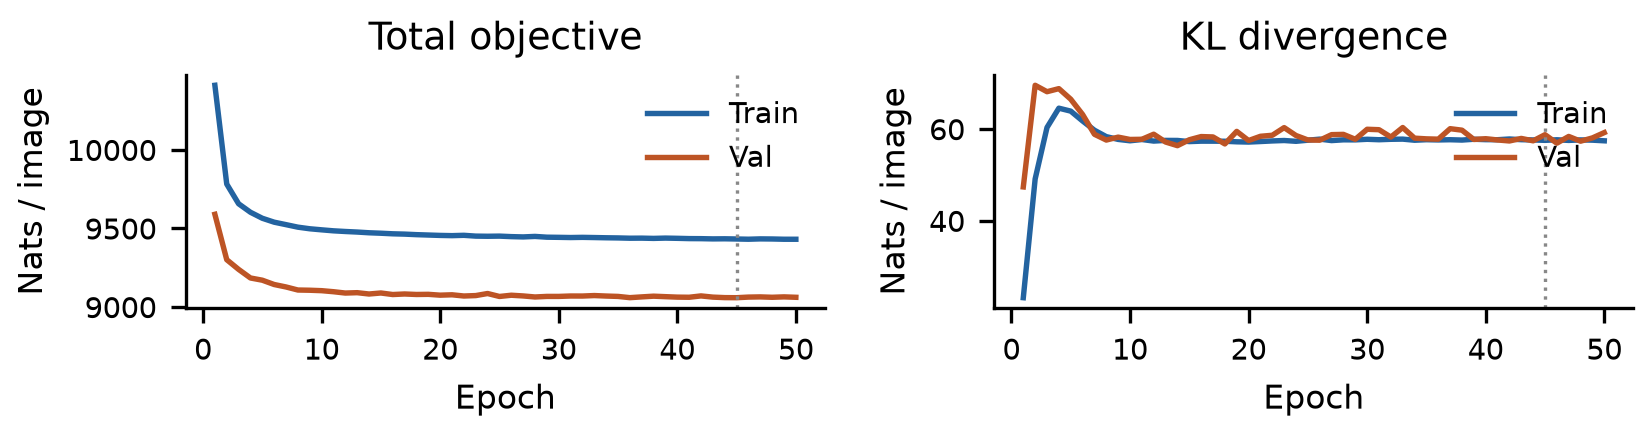
\includegraphics[width=\linewidth]{figures/training_curves.png}
\caption{Losses over 50 epochs. The dotted line marks the selected model at epoch \SelectedEpoch{}.}
\label{fig:curves}
\end{figure}

\newpage
\section{Output and Model Evaluation}
The selected decoder generates 624 images from $z\sim\mathcal N(0,I)$. Figure~\ref{fig:samples} shows the first 16 draws of real images and generated images.
\begin{figure}[h]
\centering
\begin{minipage}{0.45\linewidth}
\centering\small Real images\\[3pt]
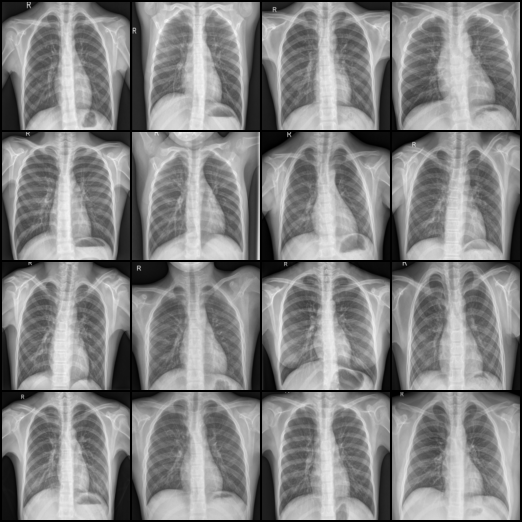
\includegraphics[width=\linewidth]{figures/real_test_grid.png}
\end{minipage}\hfill
\begin{minipage}{0.45\linewidth}
\centering\small Generated images\\[3pt]
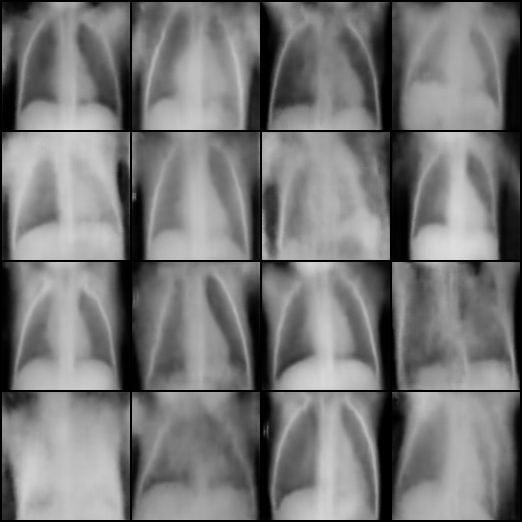
\includegraphics[width=\linewidth]{figures/generated_grid.png}
\end{minipage}
\caption{Real images (left) and generated images (right).}
\label{fig:samples}
\end{figure}

For the evaluation process, we use the inception score and FID score for generated images. Real and generated
8-bit PNGs receive the same preprocessing, which includes three identical channels, PIL bilinear
resizing to $299\times299$, and ImageNet mean or standard normalization.

Here's a summary for the evaluation metrics:

\begin{center}
\small
\begin{tabular}{lr}
\toprule
Metric (624 real / 624 generated images) & Measured value\\
\midrule
FID, pooled 2,048-D features $\downarrow$ & \FIDvalue{}\\
Inception Score, generated, full set $\uparrow$ & \ISvalue{}\\
Inception Score, generated, 10 splits (mean $\pm$ SD) & $\ISsplitmean\pm\ISsplitstd$\\
Inception Score, real test, full set (context only) & \ISreal{}\\
\bottomrule
\end{tabular}
\end{center}

\section{Limitations}
The samples preserve the overall lung outlines, but with blurred ribs and boundaries. The lower validation loss might be insufficient since the validation set contains only 16 balanced images. Also, FID’s covariance matrices are singular at $n=624$. Therefore, for future improvements, increasing the validation set and running multiple training runs with different initial weights might help with reliability and robustness.
\end{document}
